\subsection{Traditional cuts on the electron lab coordinates $\phi, \theta, p$}
The fiducial cut in the lab coordinates has been determined during the $\pi^0$ analysis in
the $\Delta(1232)$ region \cite{bib:pi0_Delta}.

Unlike the electron case, the $\phi$ boundaries are asymmetric, as shown in
Fig.~\ref{fig:proton_tph}.
\begin{figure}[h]
 \begin{center}
 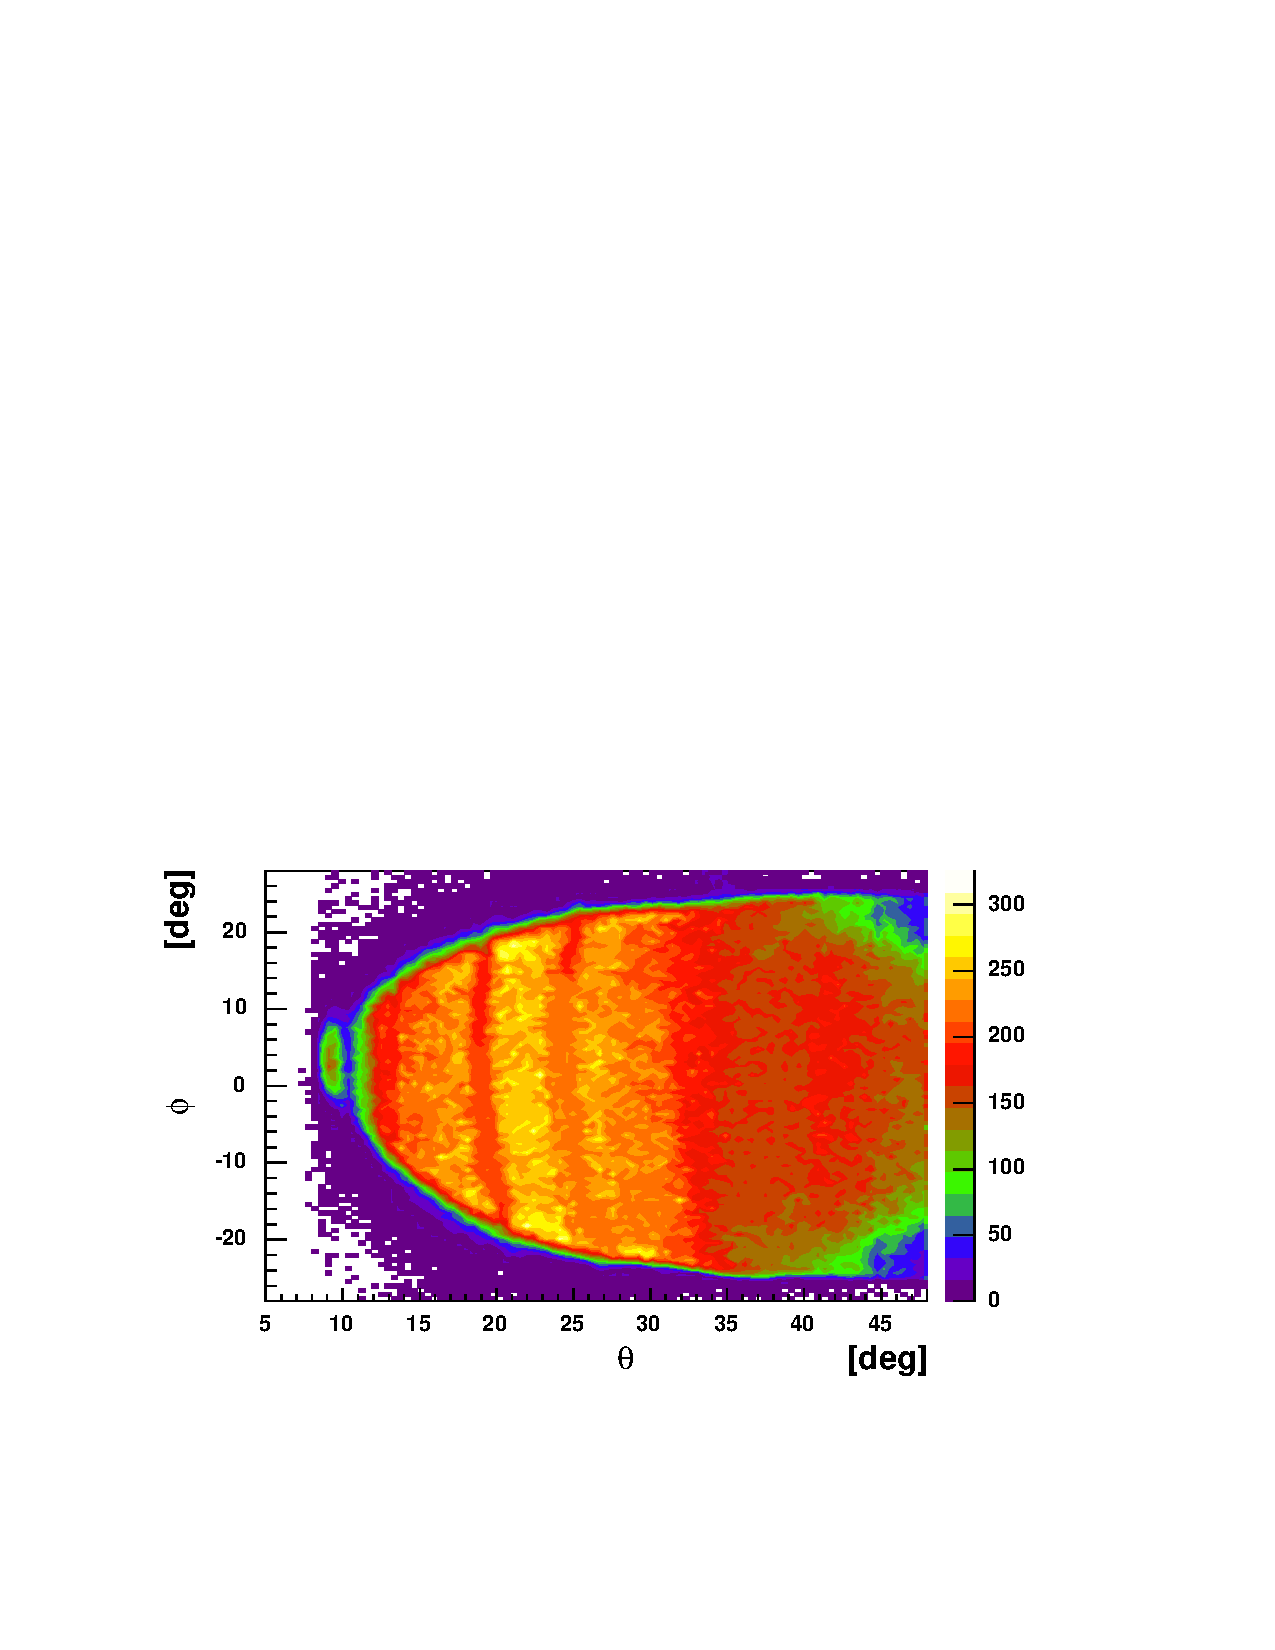
\includegraphics[width = 13cm, bb=40 120 520 420]{img/proton_tph}
  \caption[$\phi$ versus $\theta$ for sector 5 protons]
           { $\phi$ versus $\theta$ for sector 5. The momentum ranges from $0.9$
	              to $1.6$ GeV. The distribution is $\phi$-asymmetric.
                      Depletions along $\phi$ similar to the electron case are visible. }
 \label{fig:proton_tph}
 \end{center}
\end{figure}

In order to evaluate $\phi$ boundaries the momentum has been divided into momentum and $\theta$ bins,
and the distributions were fitted with the tent function shown in appendix \ref{sec:tent_function}.
An example of such fit is shown in Fig.~\ref{fig:tent_fit_s5}.

\begin{figure}[tbp]
 \begin{center}
 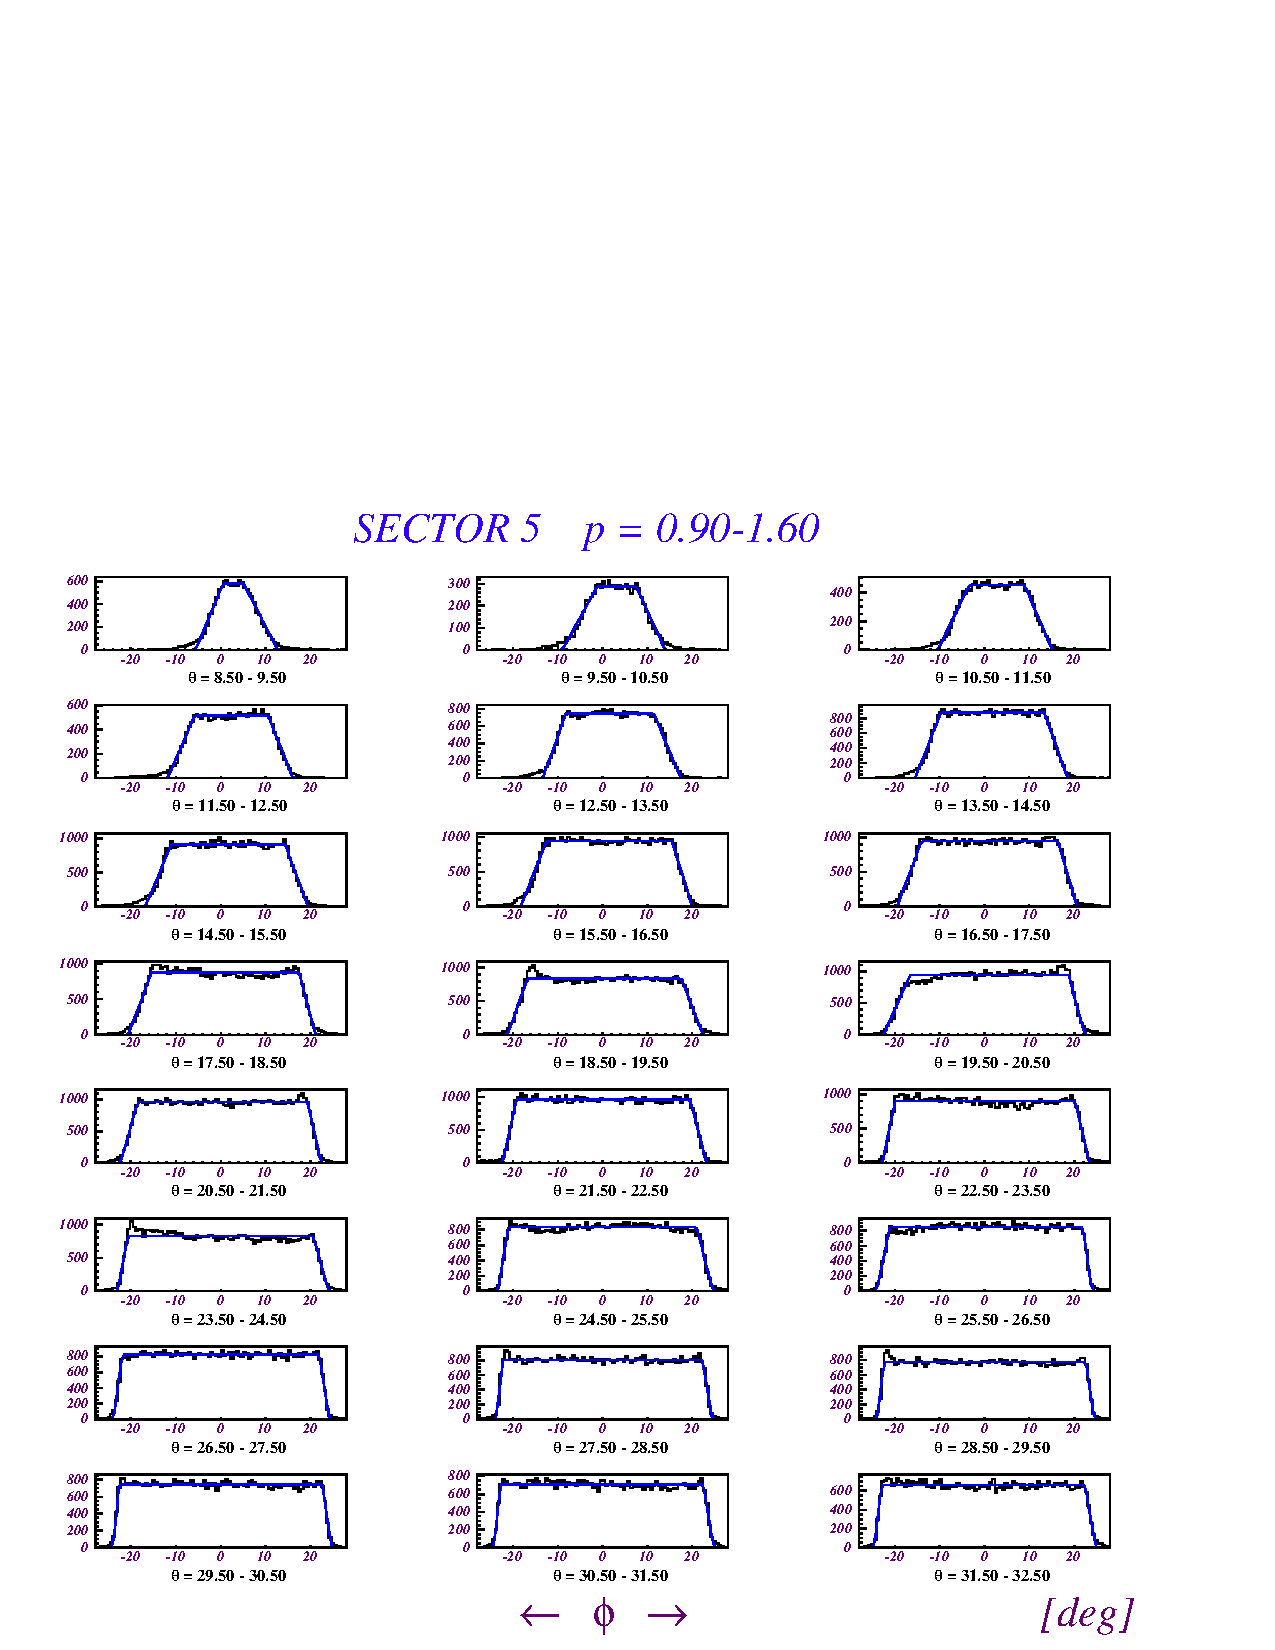
\includegraphics[width = 16cm, bb=0 0 560 560]{img/traped_fit_s5}
  \caption[Trapezoid fit for sector 5]
          { Trapezoid fit for sector 5. The limits of the flat $\phi$ region of each fit
                     will determine the fiducial cut.}
 \label{fig:traped_fit_s5}
 \end{center}
\end{figure}

The parameters are fitted as a function
of $\theta$ with a fourth order polynomial:
$$
\begin{array}{c}
 \phi_{MIN} = a_0 + a_1\theta + a_2\theta^2 + a_3\theta^3 + a_4\theta^4 \\
 \phi_{MAX} = b_0 + b_1\theta + b_2\theta^2 + b_3\theta^3 + b_4\theta^4 \\
\end{array}
$$

Fig.~\ref{fig:traped_fit_result_s5} shows the calculated $\phi_{MIN}$ and $\phi_{MAX}$  and the resulting fit
for sector 5 and momentum range $0.9$ to $1.6$ GeV.

\begin{figure}[h]
 \begin{center}
 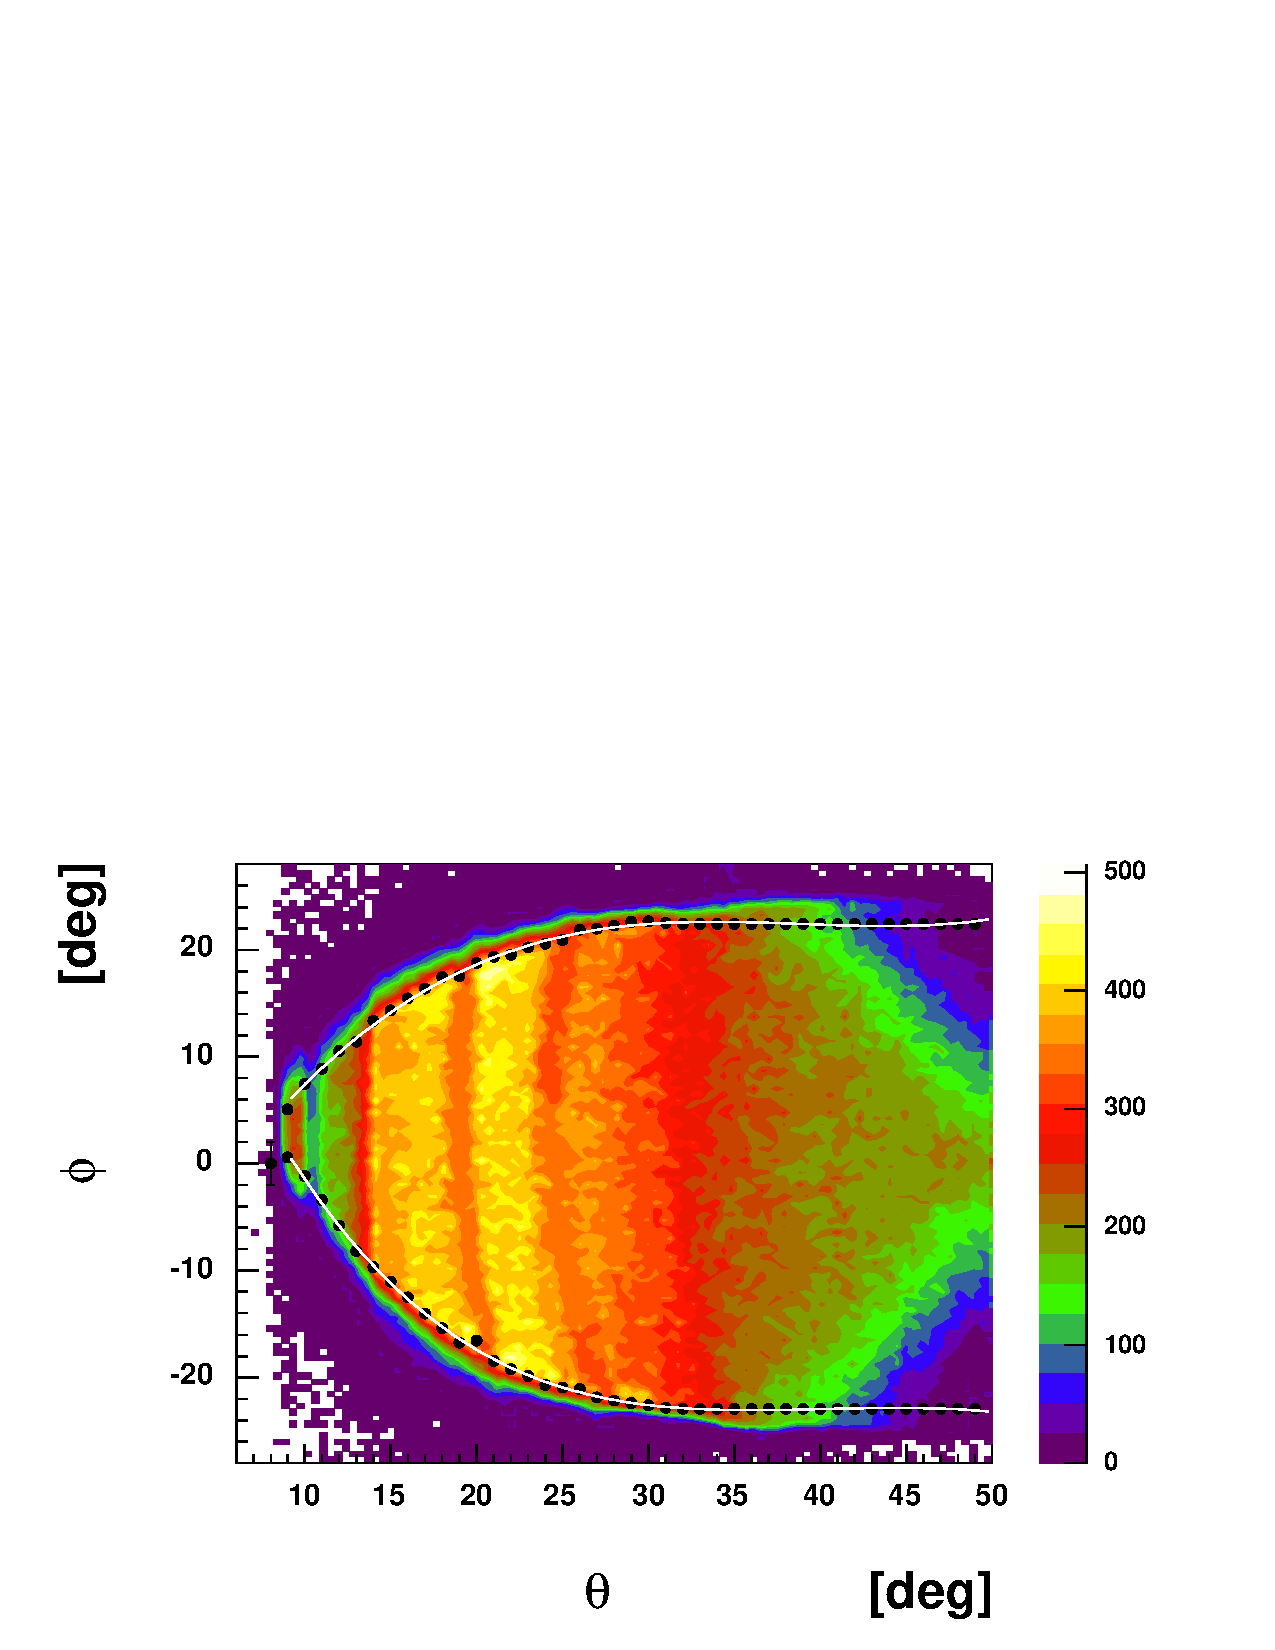
\includegraphics[width = 13cm, bb=0 0 580 430]{img/traped_fit_result_s5}
  \caption[Result of the trapezoid fit]
          { Result of the trapezoid fit for sector 5. The proton momentum ranges from $0.9$
	             to $1.6$ GeV.
	             The black points are the parameters $p_1$ (negative $\phi$) and $p_2$ (positive $\phi$)
                     for each $\theta$ slice considered as shown in Fig.~\ref{fig:traped_fit_s5}.
		     The white line is a fourth order polynomial fit to the black points.}
 \label{fig:traped_fit_result_s5}
 \end{center}
\end{figure}

\subsection{ $\theta$ versus momentum cuts}
Sector 2, 3, 5 and 6 present holes and depletions which are taken care of with the
cuts shown on Fig.~\ref{fig:proton_tp} where $\theta$ is plotted against the momentum $p$.

\begin{figure}[h]
 \begin{center}
 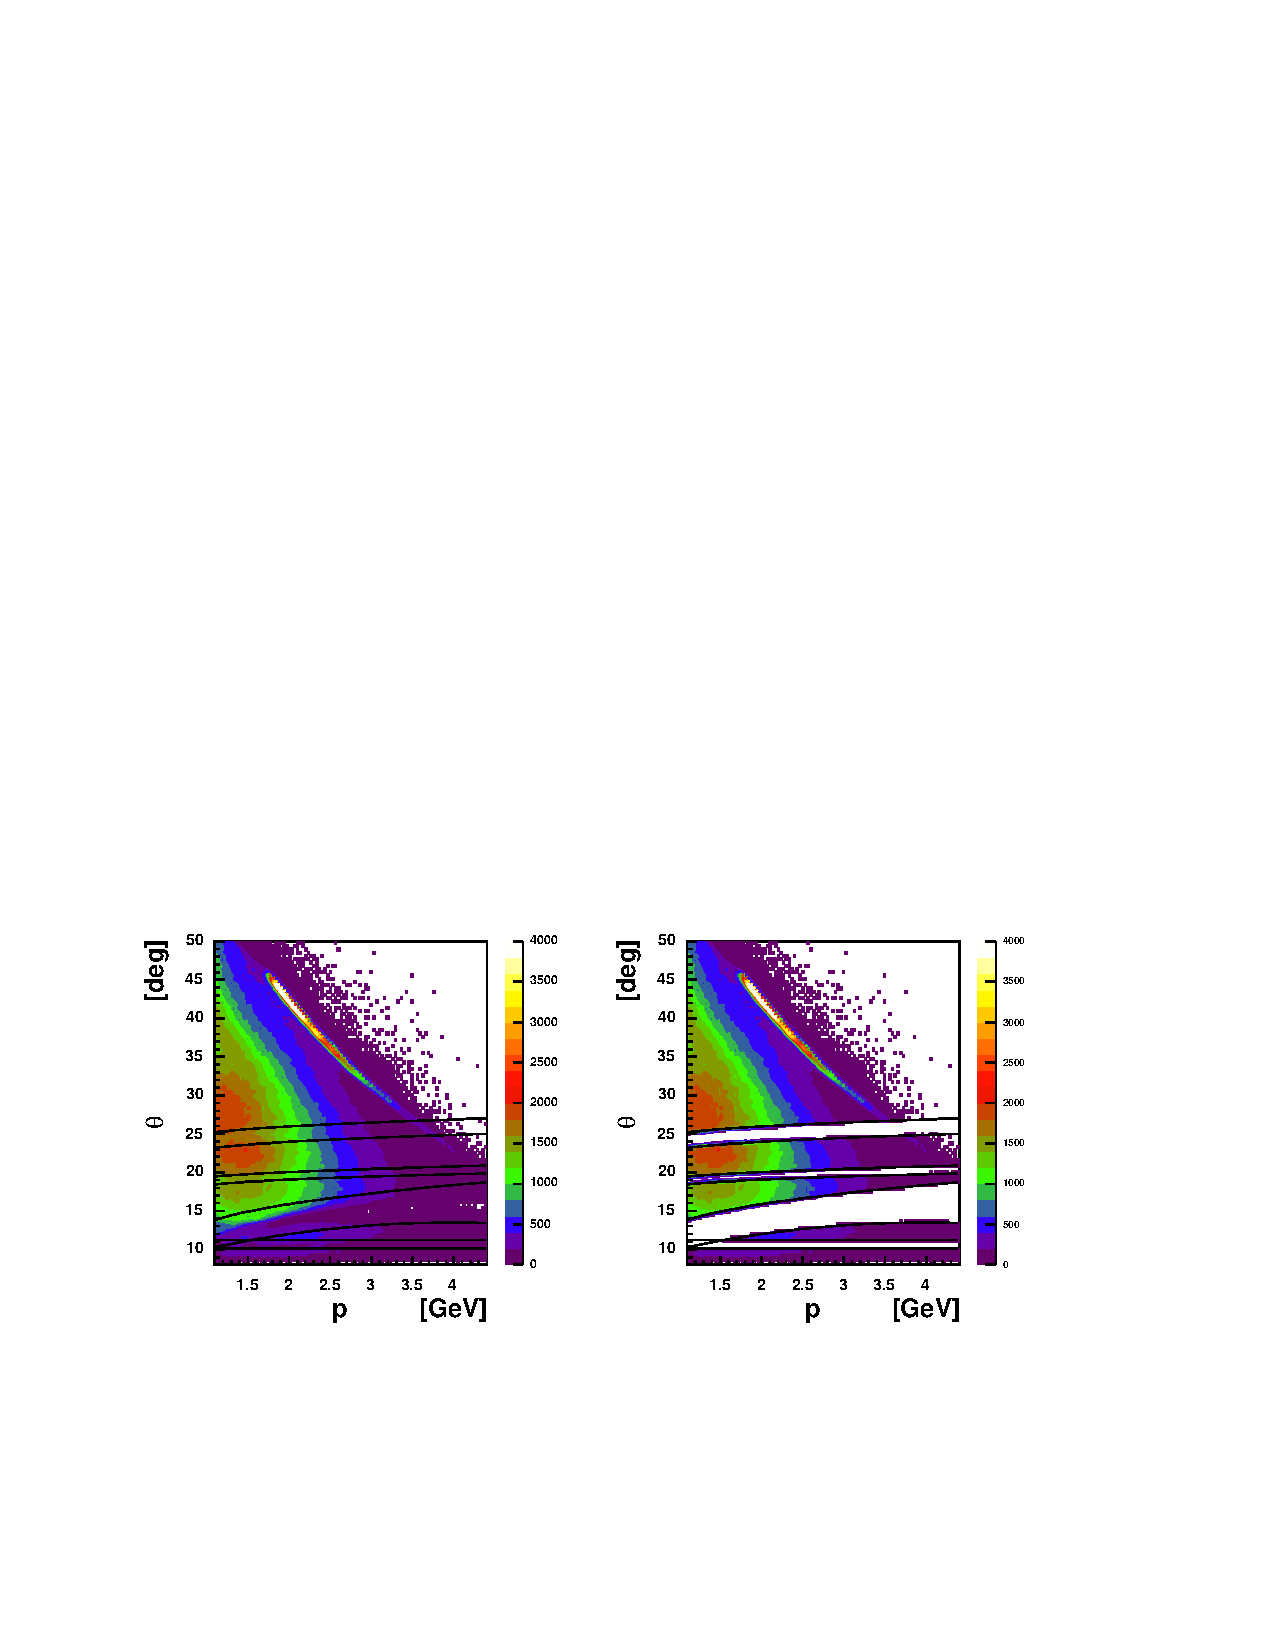
\includegraphics[width = 15cm, bb=20 140 520 380]{img/proton_tp}
  \caption[$\theta$ versus $p$ for protons sector 5]
          { $\theta$ versus $p$ for protons sector 5. A depletion is clearly visible and cut out.}
 \label{fig:proton_tp}
 \end{center}
\end{figure}


The effect of the fiducial cut on sector 5 is shown in Fig.~\ref{fig:fid_p_sector5_result}.

\begin{figure}[h]
 \begin{center}
 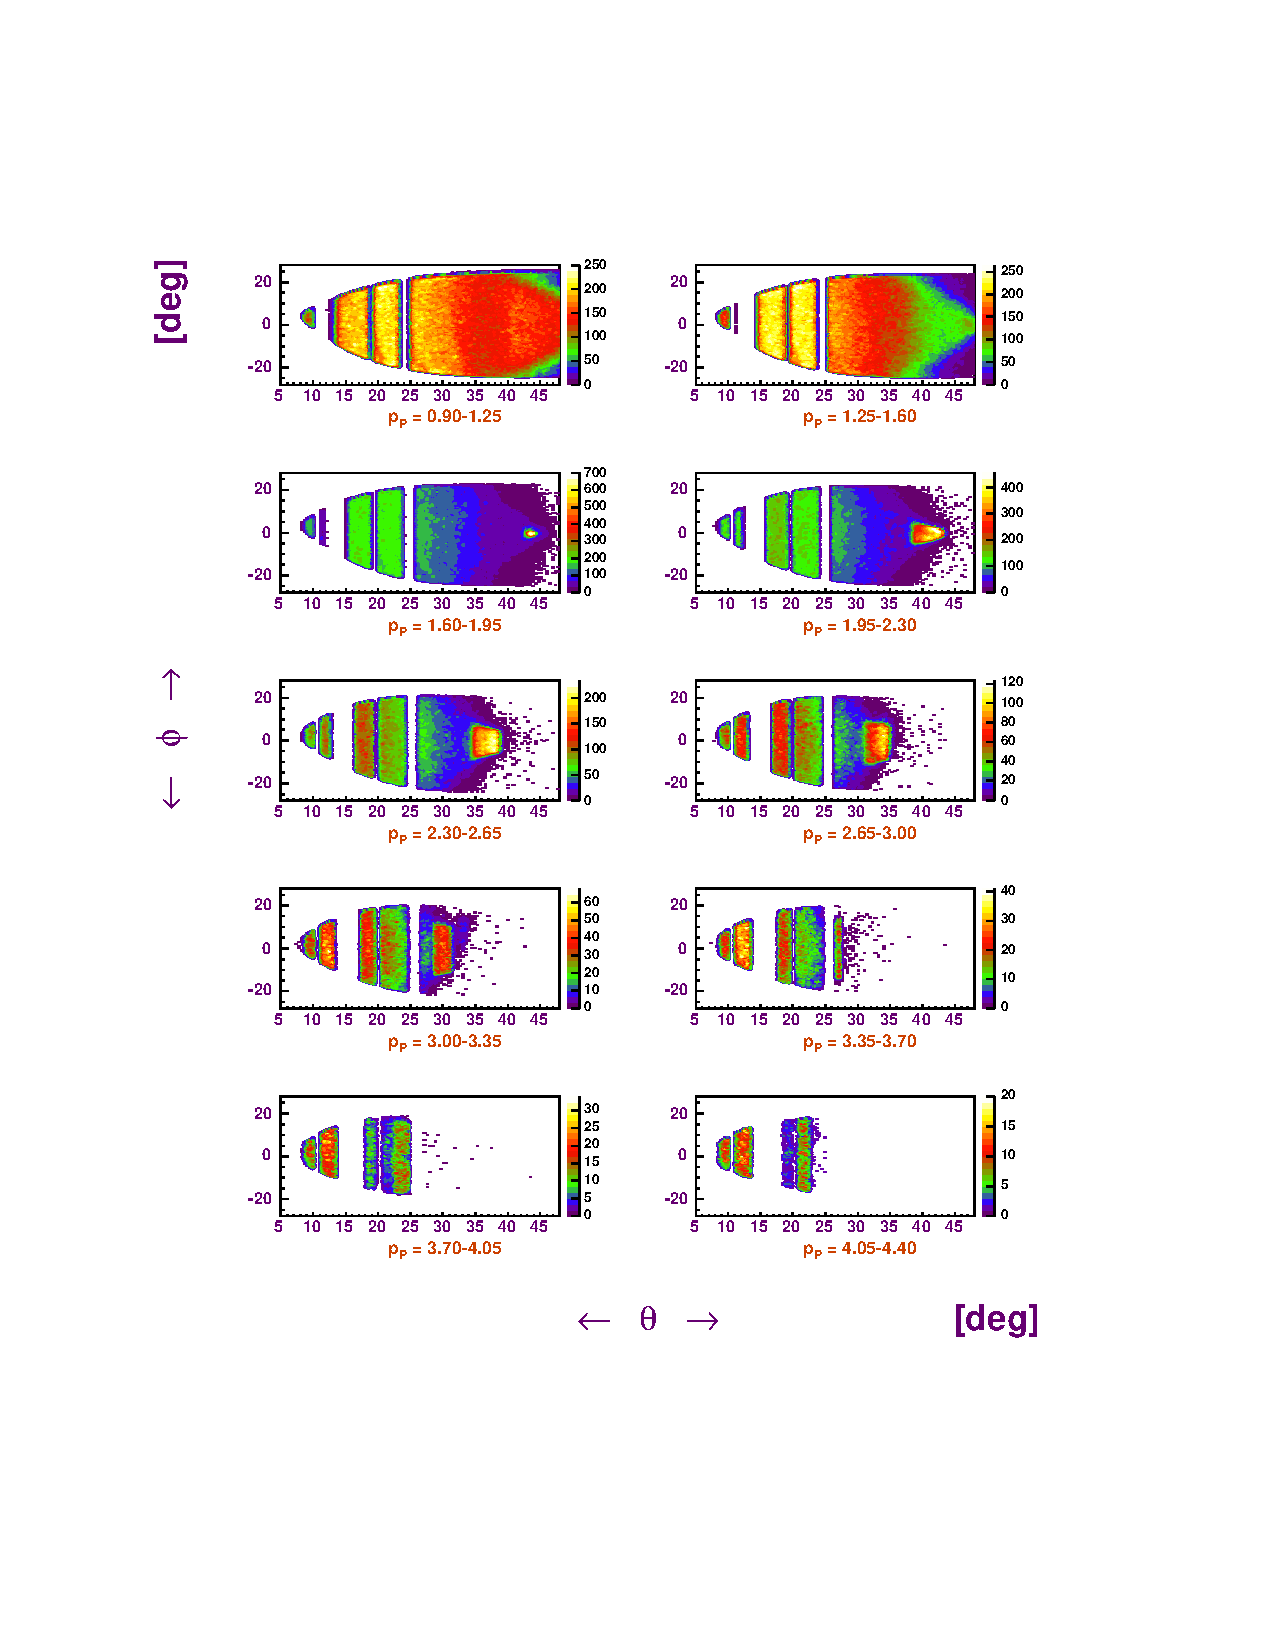
\includegraphics[width = 14cm, bb=60 140 500 660]{img/fid_p_sector5_result}
  \caption[Sector 5 $\phi$ versus $\theta$ after fiducial cut]
          { Sector 5 $\phi$ versus $\theta$ after fiducial cut. The empty bands
	             in this sector are unfortunate because the forward ones occur
		     where many protons of interest to us are expected. }
 \label{fig:fid_p_sector5_result}
 \end{center}
\end{figure}


